

\tikzset{every picture/.style={line width=0.75pt}} %set default line width to 0.75pt        

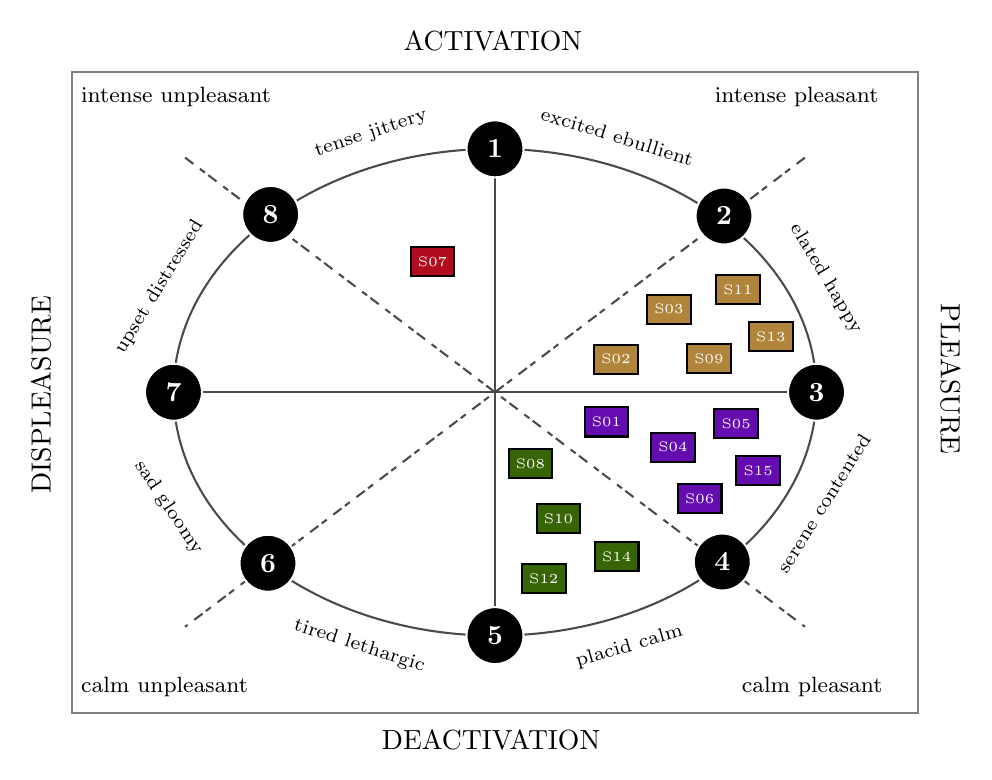
\begin{tikzpicture}[x=0.75pt,y=0.75pt,yscale=-1,xscale=1]
%uncomment if require: \path (0,389); %set diagram left start at 0, and has height of 389

%Flowchart: Or [id:dp3592995680476845] 
\draw  [color={rgb, 255:red, 74; green, 74; blue, 74 }  ,draw opacity=1 ] (182.64,181.1) .. controls (182.64,116.34) and (252,63.84) .. (337.55,63.84) .. controls (423.11,63.84) and (492.46,116.34) .. (492.46,181.1) .. controls (492.46,245.86) and (423.11,298.36) .. (337.55,298.36) .. controls (252,298.36) and (182.64,245.86) .. (182.64,181.1) -- cycle ; \draw  [color={rgb, 255:red, 74; green, 74; blue, 74 }  ,draw opacity=1 ] (182.64,181.1) -- (492.46,181.1) ; \draw  [color={rgb, 255:red, 74; green, 74; blue, 74 }  ,draw opacity=1 ] (337.55,63.84) -- (337.55,298.36) ;
%Straight Lines [id:da30798451784186187] 
\draw [color={rgb, 255:red, 74; green, 74; blue, 74 }  ,draw opacity=1 ] [dash pattern={on 3.75pt off 3pt on 2.25pt off 1.5pt}]  (188.22,68.06) -- (486.88,294.14) ;
%Straight Lines [id:da7804870395610348] 
\draw [color={rgb, 255:red, 74; green, 74; blue, 74 }  ,draw opacity=1 ] [dash pattern={on 3.75pt off 3pt on 2.25pt off 1.5pt}]  (486.88,68.06) -- (188.22,294.14) ;
%Shape: Rectangle [id:dp23344423808181314] 
\draw  [color={rgb, 255:red, 128; green, 128; blue, 128 }  ,draw opacity=1 ] (133.68,26.77) -- (541.42,26.77) -- (541.42,335.43) -- (133.68,335.43) -- cycle ;

% Text Node
\draw  [color={rgb, 255:red, 0; green, 0; blue, 0 }  ,draw opacity=1 ][fill={rgb, 255:red, 176; green, 132; blue, 58 }  ,fill opacity=1 ]  (385.29,158.22) -- (406.29,158.22) -- (406.29,172.22) -- (385.29,172.22) -- cycle  ;
\draw (395.79,165.22) node  [font=\tiny,color={rgb, 255:red, 255; green, 255; blue, 255 }  ,opacity=1 ] [align=left] {S02};
% Text Node
\draw  [color={rgb, 255:red, 0; green, 0; blue, 0 }  ,draw opacity=1 ][fill={rgb, 255:red, 176; green, 132; blue, 58 }  ,fill opacity=1 ]  (444.09,124.64) -- (465.09,124.64) -- (465.09,138.64) -- (444.09,138.64) -- cycle  ;
\draw (454.59,131.64) node  [font=\tiny,color={rgb, 255:red, 255; green, 255; blue, 255 }  ,opacity=1 ] [align=left] {S11};
% Text Node
\draw  [color={rgb, 255:red, 0; green, 0; blue, 0 }  ,draw opacity=1 ][fill={rgb, 255:red, 176; green, 132; blue, 58 }  ,fill opacity=1 ]  (410.87,134.11) -- (431.87,134.11) -- (431.87,148.11) -- (410.87,148.11) -- cycle  ;
\draw (421.37,141.11) node  [font=\tiny,color={rgb, 255:red, 255; green, 255; blue, 255 }  ,opacity=1 ] [align=left] {S03};
% Text Node
\draw  [color={rgb, 255:red, 0; green, 0; blue, 0 }  ,draw opacity=1 ][fill={rgb, 255:red, 176; green, 132; blue, 58 }  ,fill opacity=1 ]  (459.95,147.33) -- (480.95,147.33) -- (480.95,161.33) -- (459.95,161.33) -- cycle  ;
\draw (470.45,154.33) node  [font=\tiny,color={rgb, 255:red, 255; green, 255; blue, 255 }  ,opacity=1 ] [align=left] {S13};
% Text Node
\draw  [color={rgb, 255:red, 0; green, 0; blue, 0 }  ,draw opacity=1 ][fill={rgb, 255:red, 176; green, 132; blue, 58 }  ,fill opacity=1 ]  (430.12,157.99) -- (451.12,157.99) -- (451.12,171.99) -- (430.12,171.99) -- cycle  ;
\draw (440.62,164.99) node  [font=\tiny,color={rgb, 255:red, 255; green, 255; blue, 255 }  ,opacity=1 ] [align=left] {S09};
% Text Node
\draw  [color={rgb, 255:red, 0; green, 0; blue, 0 }  ,draw opacity=1 ][fill={rgb, 255:red, 100; green, 12; blue, 176 }  ,fill opacity=1 ]  (380.72,188.42) -- (401.72,188.42) -- (401.72,202.42) -- (380.72,202.42) -- cycle  ;
\draw (391.22,195.42) node  [font=\tiny,color={rgb, 255:red, 255; green, 255; blue, 255 }  ,opacity=1 ] [align=left] {S01};
% Text Node
\draw  [color={rgb, 255:red, 0; green, 0; blue, 0 }  ,draw opacity=1 ][fill={rgb, 255:red, 100; green, 12; blue, 176 }  ,fill opacity=1 ]  (443.25,189.14) -- (464.25,189.14) -- (464.25,203.14) -- (443.25,203.14) -- cycle  ;
\draw (453.75,196.14) node  [font=\tiny,color={rgb, 255:red, 255; green, 255; blue, 255 }  ,opacity=1 ] [align=left] {S05};
% Text Node
\draw  [color={rgb, 255:red, 0; green, 0; blue, 0 }  ,draw opacity=1 ][fill={rgb, 255:red, 100; green, 12; blue, 176 }  ,fill opacity=1 ]  (412.76,200.61) -- (433.76,200.61) -- (433.76,214.61) -- (412.76,214.61) -- cycle  ;
\draw (423.26,207.61) node  [font=\tiny,color={rgb, 255:red, 255; green, 255; blue, 255 }  ,opacity=1 ] [align=left] {S04};
% Text Node
\draw  [color={rgb, 255:red, 0; green, 0; blue, 0 }  ,draw opacity=1 ][fill={rgb, 255:red, 100; green, 12; blue, 176 }  ,fill opacity=1 ]  (453.83,211.83) -- (474.83,211.83) -- (474.83,225.83) -- (453.83,225.83) -- cycle  ;
\draw (464.33,218.83) node  [font=\tiny,color={rgb, 255:red, 255; green, 255; blue, 255 }  ,opacity=1 ] [align=left] {S15};
% Text Node
\draw  [color={rgb, 255:red, 0; green, 0; blue, 0 }  ,draw opacity=1 ][fill={rgb, 255:red, 100; green, 12; blue, 176 }  ,fill opacity=1 ]  (425.68,225.39) -- (446.68,225.39) -- (446.68,239.39) -- (425.68,239.39) -- cycle  ;
\draw (436.18,232.39) node  [font=\tiny,color={rgb, 255:red, 255; green, 255; blue, 255 }  ,opacity=1 ] [align=left] {S06};
% Text Node
\draw  [color={rgb, 255:red, 0; green, 0; blue, 0 }  ,draw opacity=1 ][fill={rgb, 255:red, 55; green, 100; blue, 4 }  ,fill opacity=1 ]  (344.1,208.52) -- (365.1,208.52) -- (365.1,222.52) -- (344.1,222.52) -- cycle  ;
\draw (354.6,215.52) node  [font=\tiny,color={rgb, 255:red, 255; green, 255; blue, 255 }  ,opacity=1 ] [align=left] {S08};
% Text Node
\draw  [color={rgb, 255:red, 0; green, 0; blue, 0 }  ,draw opacity=1 ][fill={rgb, 255:red, 55; green, 100; blue, 4 }  ,fill opacity=1 ]  (357.61,234.99) -- (378.61,234.99) -- (378.61,248.99) -- (357.61,248.99) -- cycle  ;
\draw (368.11,241.99) node  [font=\tiny,color={rgb, 255:red, 255; green, 255; blue, 255 }  ,opacity=1 ] [align=left] {S10};
% Text Node
\draw  [color={rgb, 255:red, 0; green, 0; blue, 0 }  ,draw opacity=1 ][fill={rgb, 255:red, 55; green, 100; blue, 4 }  ,fill opacity=1 ]  (385.68,253.21) -- (406.68,253.21) -- (406.68,267.21) -- (385.68,267.21) -- cycle  ;
\draw (396.18,260.21) node  [font=\tiny,color={rgb, 255:red, 255; green, 255; blue, 255 }  ,opacity=1 ] [align=left] {S14};
% Text Node
\draw  [color={rgb, 255:red, 0; green, 0; blue, 0 }  ,draw opacity=1 ][fill={rgb, 255:red, 55; green, 100; blue, 4 }  ,fill opacity=1 ]  (350.53,263.78) -- (371.53,263.78) -- (371.53,277.78) -- (350.53,277.78) -- cycle  ;
\draw (361.03,270.78) node  [font=\tiny,color={rgb, 255:red, 255; green, 255; blue, 255 }  ,opacity=1 ] [align=left] {S12};
% Text Node
\draw  [color={rgb, 255:red, 0; green, 0; blue, 0 }  ,draw opacity=1 ][fill={rgb, 255:red, 176; green, 11; blue, 31 }  ,fill opacity=1 ]  (296.94,111.16) -- (317.94,111.16) -- (317.94,125.16) -- (296.94,125.16) -- cycle  ;
\draw (307.44,118.16) node  [font=\tiny,color={rgb, 255:red, 255; green, 255; blue, 255 }  ,opacity=1 ] [align=left] {S07};
% Text Node
\draw  [color={rgb, 255:red, 255; green, 255; blue, 255 }  ,draw opacity=1 ][fill={rgb, 255:red, 0; green, 0; blue, 0 }  ,fill opacity=1 ]  (337.55, 63.84) circle [x radius= 13.73, y radius= 13.73]   ;
\draw (337.55,63.84) node  [font=\normalsize,color={rgb, 255:red, 255; green, 255; blue, 255 }  ,opacity=1 ] [align=left] {\textbf{1}};
% Text Node
\draw  [color={rgb, 255:red, 255; green, 255; blue, 255 }  ,draw opacity=1 ][fill={rgb, 255:red, 0; green, 0; blue, 0 }  ,fill opacity=1 ]  (447.88, 96.18) circle [x radius= 13.73, y radius= 13.73]   ;
\draw (447.88,96.18) node  [font=\normalsize,color={rgb, 255:red, 255; green, 255; blue, 255 }  ,opacity=1 ] [align=left] {\textbf{2}};
% Text Node
\draw  [color={rgb, 255:red, 255; green, 255; blue, 255 }  ,draw opacity=1 ][fill={rgb, 255:red, 0; green, 0; blue, 0 }  ,fill opacity=1 ]  (492.46, 181.1) circle [x radius= 13.73, y radius= 13.73]   ;
\draw (492.46,181.1) node  [font=\normalsize,color={rgb, 255:red, 255; green, 255; blue, 255 }  ,opacity=1 ] [align=left] {\textbf{3}};
% Text Node
\draw  [color={rgb, 255:red, 255; green, 255; blue, 255 }  ,draw opacity=1 ][fill={rgb, 255:red, 0; green, 0; blue, 0 }  ,fill opacity=1 ]  (447.05, 262.88) circle [x radius= 13.73, y radius= 13.73]   ;
\draw (447.05,262.88) node  [font=\normalsize,color={rgb, 255:red, 255; green, 255; blue, 255 }  ,opacity=1 ] [align=left] {\textbf{4}};
% Text Node
\draw  [color={rgb, 255:red, 255; green, 255; blue, 255 }  ,draw opacity=1 ][fill={rgb, 255:red, 0; green, 0; blue, 0 }  ,fill opacity=1 ]  (337.55, 298.36) circle [x radius= 13.73, y radius= 13.73]   ;
\draw (337.55,298.36) node  [font=\normalsize,color={rgb, 255:red, 255; green, 255; blue, 255 }  ,opacity=1 ] [align=left] {\textbf{5}};
% Text Node
\draw  [color={rgb, 255:red, 255; green, 255; blue, 255 }  ,draw opacity=1 ][fill={rgb, 255:red, 0; green, 0; blue, 0 }  ,fill opacity=1 ]  (228.16, 263.49) circle [x radius= 13.73, y radius= 13.73]   ;
\draw (228.16,263.49) node  [font=\normalsize,color={rgb, 255:red, 255; green, 255; blue, 255 }  ,opacity=1 ] [align=left] {\textbf{6}};
% Text Node
\draw  [color={rgb, 255:red, 255; green, 255; blue, 255 }  ,draw opacity=1 ][fill={rgb, 255:red, 0; green, 0; blue, 0 }  ,fill opacity=1 ]  (182.64, 181.1) circle [x radius= 13.73, y radius= 13.73]   ;
\draw (182.64,181.1) node  [font=\normalsize,color={rgb, 255:red, 255; green, 255; blue, 255 }  ,opacity=1 ] [align=left] {\textbf{7}};
% Text Node
\draw  [color={rgb, 255:red, 255; green, 255; blue, 255 }  ,draw opacity=1 ][fill={rgb, 255:red, 0; green, 0; blue, 0 }  ,fill opacity=1 ]  (229.45, 95.43) circle [x radius= 13.73, y radius= 13.73]   ;
\draw (229.45,95.43) node  [font=\normalsize,color={rgb, 255:red, 255; green, 255; blue, 255 }  ,opacity=1 ] [align=left] {\textbf{8}};
% Text Node
\draw (112.89,231.39) node [anchor=north west][inner sep=0.75pt]  [rotate=-270] [align=left] {DISPLEASURE};
% Text Node
\draw (292.08,5.96) node [anchor=north west][inner sep=0.75pt]   [align=left] {ACTIVATION};
% Text Node
\draw (281.58,342.71) node [anchor=north west][inner sep=0.75pt]   [align=left] {DEACTIVATION};
% Text Node
\draw (562.94,136.89) node [anchor=north west][inner sep=0.75pt]  [rotate=-90] [align=left] {PLEASURE};
% Text Node
\draw (150.9,160.23) node [anchor=north west][inner sep=0.75pt]  [font=\scriptsize,rotate=-301.49] [align=left] {upset distressed};
% Text Node
\draw (247.79,60.45) node [anchor=north west][inner sep=0.75pt]  [font=\scriptsize,rotate=-341.6] [align=left] {tense jittery};
% Text Node
\draw (359.94,41.46) node [anchor=north west][inner sep=0.75pt]  [font=\scriptsize,rotate=-17.34] [align=left] {excited ebullient};
% Text Node
\draw (485.75,96.5) node [anchor=north west][inner sep=0.75pt]  [font=\scriptsize,rotate=-59.2] [align=left] {elated happy};
% Text Node
\draw (470.66,265.95) node [anchor=north west][inner sep=0.75pt]  [font=\scriptsize,rotate=-301.93] [align=left] {serene contented};
% Text Node
\draw (373.68,306.2) node [anchor=north west][inner sep=0.75pt]  [font=\scriptsize,rotate=-343.65] [align=left] {placid calm};
% Text Node
\draw (241.21,287.33) node [anchor=north west][inner sep=0.75pt]  [font=\scriptsize,rotate=-18.04] [align=left] {tired lethargic};
% Text Node
\draw (169.56,210.51) node [anchor=north west][inner sep=0.75pt]  [font=\scriptsize,rotate=-56.13] [align=left] {sad gloomy};
% Text Node
\draw (455,317) node [anchor=north west][inner sep=0.75pt]  [font=\footnotesize] [align=left] {calm pleasant};
% Text Node
\draw (136.67,317) node [anchor=north west][inner sep=0.75pt]  [font=\footnotesize] [align=left] {calm unpleasant};
% Text Node
\draw (136.67,32.78) node [anchor=north west][inner sep=0.75pt]  [font=\footnotesize] [align=left] {intense unpleasant};
% Text Node
\draw (442,32.78) node [anchor=north west][inner sep=0.75pt]  [font=\footnotesize] [align=left] {intense pleasant};


\end{tikzpicture}
